\documentclass[a4paper,12 pt,twoside]{report}
\usepackage{fullpage}

\usepackage{mystyle}
\pagenumbering{arabic}

\begin{document}

\begin{titlepage}

  % AUTH Logo
  \begin{minipage}{0.3\textwidth}
    \begin{flushleft}
      
\includegraphics[scale=0.25]{./images/title/authLogoTr.jpg}
    \end{flushleft}
  \end{minipage}
  \begin{minipage}{0.9\textwidth}
    \begin{flushleft}
      \large Αριστοτέλειο Πανεπιστήμιο Θεσσαλονίκης \\
      Πολυτεχνική Σχολή \\
      Τμήμα Ηλεκτρολόγων Μηχανικών $\&$ \\ Μηχανικών Υπολογιστών\\

      \normalsize{Τομέας Ηλεκτρονικής και Υπολογιστών} \\[5cm]
    \end{flushleft}
  \end{minipage} \\[1.7cm]




  \begin{center}
    \Large Διπλωματική Εργασία \\[0.8cm]

    \rule{450pt}{4pt} \\[0.4cm]
    {\fontsize{20.26pt}{1em}\selectfont Σύστημα για την Αυτόματη Παρακολούθηση του Χρόνου Λειτουργίας και Απόκρισης ενός Ιστότοπου}

    \rule{350pt}{4pt} \\[4cm]

    % Writer
    \begin{minipage}{0.4\textwidth}
      \begin{flushleft} \normalsize
        \emph{Εκπόνηση:} \\
        Σεντονάς Σταύρος \\
        ΑΕΜ: 9386
      \end{flushleft}
    \end{minipage}
    % Supervisors
    \begin{minipage}{0.4\textwidth}
      \begin{flushright} \normalsize
        \emph{Επίβλεψη:} \\
        Υπ. Δρ. Καρανικιώτης Θωμάς \\
        Δρ. Παπαμιχαήλ Μιχαήλ \\
        Καθ. Συμεωνίδης Ανδρέας\\
      \end{flushright}
    \end{minipage}
    \\[1cm]
    \vfill

    % Title
    \large Θεσσαλονίκη, Ιούνιος 2023

  \end{center}
\end{titlepage}


\newevenside

\begin{center}
  \centering

  \vspace{0.5cm}
  \centering
  \textbf{\Large{Περίληψη}}
  \phantomsection
  \addcontentsline{toc}{section}{Περίληψη}

  \vspace{1cm}

\end{center}

  Η εξέλιξη της τεχνολογίας και της πληθώρας εφαρμογών που αναπτύσσονται στα πλαίσιο αυτής, καθιστούν επιτακτική την ανάγκη ύπαρξης συστημάτων που θα ελέγχουν την εύρυθμη λειτουργία τους. Πιο συγκεκριμένα μιλάμε για την ελέξιλη στο χώρο του διαδικτύου και των δομών που έχουν υλοποιηθεί πάνω σε αυτό.
  
  Πλέον αναφερόμαστε σε ένα συνεχώς αυξανόμενο και ευρύ δίκτυο web εφαρμογών - λογισμικών ως υπηρεσίες (SaaS - Software as a Service) που ζουν στον Διαδίκτυο (World Wide Web). H λειτουργία αυτών μπορεί να ελεχθεί με διάφορους τρόπους. Από Unit Testing, στο πλαίσιο του κύκλου ανάντυξης του λογισμικού (continuous integration, continuous deployment cycle) προκειμένου να ελεχθεί λειτουργικά το σύστημα για την αποφυγή bugs, μέχρι και Παρακολούθηση Δικτύου (Network Monitoring), για να επιβεβαιωθεί η σωστή λειτουργία των συστημάτων καθόλη της διάρκεια του κύκλου ζωής τους.
  
  Η παρούσα διπλωματική εστιάζει στην ανάπτυξη ενός συστήματος Παρακολούθησης Δικτύου και κατεπέκταση εφαρμογής που θα παρέχει τη δυνατότητα στους χρήστες της να παρακολουθούν, εύκολα, την ομαλή λειτουργία των διαδικτυακών σελιδών τους, είτε αυτά είναι εφαρμογές, είτε απλά στατικές σελίδες. Το σύστημα στηρίζεται στη βασική μέθοδο εντοπισμού διαθεσιμότητας μίας ιστοσελίδας, γνωστή και ως ping. Κάνοντας ping μπορούμε να πάρουμε χρήσιμη πληροφορία σχετικά με το αν το υπό μελέτη σύστημα μπορεί να αποκριθεί ορθά στα αιτήματα που δέχεται, και σχετικά με το χρόνο που χρειάστηκε προκειμένου να απαντήσει. Συνεχίζοντας την λογική πορεία ενός τέτοιου συστήματος μπορούμε ακόμα στο μήνυμα που στέλνουμε να έχουμε πληροφορία που θα επηρεάζει την απάντηση που θα περιμέναμε να δούμε, έχοντας έτσι έναν ακόμα μηχανισμό για την αναγνώριση και αποφυγή πιθανών bugs, ή λαθών κατά τη διαδικασία ανάπτυξης λογισμικών ως υπηρεσία.

\newevenside
{\fontfamily{cmr}\selectfont

\phantomsection
\addcontentsline{toc}{section}{Abstract}


\begin{center}
  \centering
  \textbf{\Large{Title}}
  \vspace{0.5cm}

  \textbf{\large{Development of an Active Monitoring System for Web Applications}}
  \vspace{1cm}

  \centering
  \textbf{Abstract}
\end{center}

The continuous digitization of daily life, has led to a plethora of internet applications developed within this framework. These data make it imperative, to have systems that will control the smooth operation of such software applications, which function as services (SaaS - Software as a Service).

Control checks can be exerted at various levels, from unit tests within the software development cycle (continuous integration, continuous deployment cycle) to Network Monitoring during the actual system operation.

While there are several tools for application control during the software development phase, there are not similarly many user-friendly and capable tools for control during the operational phase. Therefore, this thesis focuses on developing an Intelligent Monitoring system and, by extension, an application that will allow users to easily monitor the smooth operation of their internet pages, whether they are applications or simple static pages, to recognize and detect abnormal operation and to automatically modify the available computational resources in real-time.

The system relies on the basic method of detecting the availability of a website, known as ping. By pinging, we obtain useful information about whether the system under study can respond correctly to the requests it receives and the time it takes to respond. Continuing the logical progression of such system, we can even modify the message we send with predetermined data, to check the response of the system and verify response, thus having an additional mechanism of identifying and avoiding potential bugs or errors during the software’s development process.

Furthermore, by analyzing the sequence of timestamps generated by continuous requests to the system under study, we can extract significant information about its evolution over time, and this way identify abnormal behaviours. Finally, if the system we study is built as a Docker container, we can even dynamically modify the available resources, in order to operate optimally even under high load conditions.


\begin{flushright}
  \vspace{2cm}
  Sentonas Stavros
  \\
  Electrical \& Computer Engineering Department,
  \\
  Aristotle University of Thessaloniki, Greece
  \\
  March 2024
\end{flushright}

}

\newevenside

\renewcommand*\contentsname{Περιεχόμενα}
\setcounter{tocdepth}{2}

\tableofcontents

\renewcommand{\listfigurename}{Κατάλογος Σχημάτων}
\listoffigures

\renewcommand{\listtablename}{Κατάλογος Πινάκων}
\listoftables

% \listoftables
% \listofalgorithms

%\listofequations
%\newlistof{myequations}{equ}{\listequationsname}
%\listofmyequations

\chapter*{Ακρωνύμια Εγγράφου}
\label{append:acronyms}
\phantomsection
\addcontentsline{toc}{section}{Ακρωνύμια}

Παρακάτω παρατίθενται ορισμένα από τα πιο συχνά χρησιμοποιούμενα ακρωνύμια της
παρούσας διπλωματικής εργασίας:

\begin{table}[htpb]
  \centering
  \begin{tabular}{l@{$\;\;\longrightarrow\;\;$}l}
	RUM & Real User Monitoring \\
  API & Application Programming Interface \\
  SaaS & Software as a Service \\
  HTTP & Hypertext Transfer Protocol \\
    % OS & Operating System \\
	% CNN & Convolutional Neural Network \\
    % CPU & Central Processing Unit \\
    % GPU & Graphics Processing Unit \\
  \end{tabular}
\end{table}



\newevenside

% %  chapter 1 = Θεώρηση Προβλήματος
% Aναφορά σε Active, Passive, Mixed Uptime monitoring
% Κίνητρο - Χρηστικότητα

\chapter{Εισαγωγή}
\label{chapter:intro}

Τα τελευταία χρόνια, ο κλάδος του Διαδικτύου προσεγγίζει ένα μεγαλύτερο κομμάτι ανθρώπων, τόσο από τη μεριά του καταναλωτή 
όσο και από τη μεριά του παραγωγού. Όσο αφορά τον καταναλωτή οι δυνατότητες που του προσφέρονται μπορούν να διακριθούν στους εξής τομέις:

\begin{itemize}
	\item Επικοινωνία: το διαδίκτυο παρέχει τη δυνατότητα άμεσης επικοινωνίας μεταξύ μεγάλων αποστάσεων, που δεν περιορίζεται μόνο στο ακουστικό
			ερέθισμα, αλλά επιτρέπει και την μετάδοση οπτικο-ακουστικής πληροφορίας
	\item Πρόσβαση Πληροφορίας: ίσως το σημεντικότερο αγαθό που προσφέρει το διαδίκτυο είναι η πληθώρα πληροφορίας
			που στεγάζει. Μηχανές Αναζήτηση (search engines), Online Βάσεις Δεδομένων (online databases),
			και άλλου είδους εφαρμογών εκπαιδευτικού χαρακτήρα που δίνουν πρόσβαση σε άτομα που το επιθυμούν, να κάνουν έρευνα
	\item Ποιότητα ζωής: σε αυτή την κατηγορία περιλαμβάνονται όλες εκείνες οι υπηρεσίες που
			διευκολύνουν την καθημερινότητα των χρηστών. Online αγορές (eshops) που γλιτώνουν την αναμονή σε ουρές ή ακόμα
			επιτρέπουν την εύκολη αγορά προϊόντων από απομακρυσμένες περιοχές του πλανήτη, ψυχαγωγία και πρόσβαση σε
			υπηρεσίες που επιταχύνουν ενέργειες που υπό άλλες περιπτώσεις θα ήταν χρονοβόρες (online banking,
			πληρωμή λογαριασμών, κρατήσεις ξενοδοχείων/εισητηρίων)
\end{itemize}

Από τη μεριά του παραγωγού, τα μέσα που υπάρχουν για την ανάπτυξη τέτοιων εφαρμογών/υπηρεσιών/συστημάτων
μέρα με τη μέρα αυξάνονται. Η ραγδαία εξέλιξη στον χώρο των cloud υποδομών, καθιστά ευκολότερη και επισπεύδει
τόσο την δημιουργία διαδικτυακών εφαρμογών, και σελιδών σε ένα γενικότερο πλαίσιο, όσο και την μεγέθυνση και αύξηση αυτών (scale up).
Μάλιστα η επιλογή κατάλληλου παρόχου τέτοιων υπηρεσιών αποτελεί ένα αρκετά σημεντικό αντικείμενο μελέτης \cite{cloud_service_provider_evaluation}.
Πέρα από τον οικομικό παράγοντα θα πρέπει να προσμετρηθούν οι παροχές, τα πλεονεκτήματα αλλά και η αποδοτικότητα που κάθε ένας προσφέρει.

Βλέποντας λοιπόν το πόσο συνυφασμένη είναι η ζωή του σύγχρονου ανθρώπου με το δίκτυο αλλά και τις δυνατότητες και τα μέσα
που έχει ο καθένας για να αναπτύξει εφαρμογές σε αυτό, καθίσταται επιτακτική η ανάγκη ύπαρξης μηχανισμών 
που θα αναγνωρίζουν σφάλματα (bugs) και θα επιβλέπουν την ορθή λειτουργία των υπό μελέτη συστημάτων καθόλη τη διάρκεια ζωής τους.

\section{Περιγραφή του Προβλήματος}
\label{section:problem_description}

Η Παρακολούθηση (Monitoring) ενός συστήματος που "ζει" στο χώρο του διαδικτύου μπορεί να γίνει κυρίως με δύο τρόπους:

\begin{itemize}
	\item \textbf{Ενεργή Παρακολούθηση (Active Monitoring)}: έχει περισσότερο προγνωστικό και προληπτικό χαρακτήρα.
		Συχνά αναφέρεται και ως \textbf{Συνθετική παρακολούθηση (Synthetic Monitoring)}, λόγω της φύσης των ενεργειών της.
		Ουσιαστικά δημιουργεί πλασματικά api calls και όχι πραγματικά δεδομένα χρηστών 
		προκειμένου να ελεγχθεί η απόκριση του υπό μελέτη συστήματος. Η συχνότητα αποστολής των
		συνθετικών αιτημάτων συνήθως ρυθμίζεται από το χρήστη.
	\item \textbf{Παθητική Παρακολούθηση (Passive Monitoring)}: παρέχει μία πιο πλήρη εικόνα σχετικά με πως χρησιμοποιούνται οι πόροι του δικτύου
		καταγράφοντας, αποθηκεύοντας και αναλύοντας τα δεδομένα του χρήστη. Για αυτό πολλές φορές αναφέρεται στη βιβλιογραφία ως \textbf{Παρακολούθηση Πραγματικών Χρηστών (Real User Monitoring - RUM)}. Έτσι μπορεί κανείς
		να εντοπίσει τις τάσεις χρήσης του δικτύου για τη βελτίωση και βελτιστοποίησή του συστήματος.
\end{itemize}


\begin{table}[H]
	\begin{center}
		\caption{Χαρακτηριστικά Ενεργής και Παθητικής Παρακολούθησης}
		\label{tab:active_vs_passive_monitoring}
		\begin{tabular}{ | c | c | }
			\hline
				\thead{Ενεργή Παρακολούθση \\ (Active Monitoring)} & \thead{Παθητική Παρακολούθηση \\ (Passive Monitoring)} \\
			\hline
				% \makecell{$\bullet$ Παράγει μικρή ποσότητα \\ δεδομένων} & \makecell{$\bullet$ Παράγει μεγάλη ποσότητα \\ δεδομένων} \\
				\makecell{$\bullet$ Στηρίζεται σε συνθετικά \\ API calls} & \makecell{$\bullet$ Αναλύει δεδομένα πραγματικών \\ χρηστών} \\
				\makecell{$\bullet$ Παράγει δεδομένα για συγκεκριμένες \\ πτυχές του δικτύου} & \makecell{$\bullet$ Πλήρης εικόνα της απόδοσης \\ του δικτύου} \\
				\makecell{$\bullet$ Μπορεί να μετρήσει την κίνηση \\ εντός και εκτός του δικτύου} & \makecell{$\bullet$ Μετράει κίνηση μόνο \\ εντός του δικτύου} \\
				\makecell{$\bullet$ Μπορεί να εντοπίσει προβλήματα \\ πριν ακόμα μπορέσουν να τα \\ εντοπίσουν οι χρήστες} & \makecell{$\bullet$ Εντοπίζει προβλήματα που \\ εμφανίζονται εκείνη τη στιγμή} \\
			\hline
		\end{tabular}
	\end{center}
\end{table}

Και οι δύο μέθοδοι έχουν πλεονεκτήματα και μειονεκτήματα, τα οποία φαίνονται και στον παραπάνω πίνακα \ref{tab:active_vs_passive_monitoring}. Όπως είναι εμφανές
η παθητική παρακολούθηση γίνεται πάνω στο σύστημα που θέλουμε να μελετήσουμε, πράγμα το οποίο σήμαινει ότι σαν εξωτερικοί παράγοντες στο
σύστημα δεν θα μπορέσουμε να προσφέρουμε ανάλογες υπηρεσίες. Για το λόγο αυτό συνεχίζουμε την ανάλυση στο πλαίσιο της Ενεργής Παρακολούθησης Δικτύων.

Οι βασικοί λόγοι που χρειάζονται τέτοιου είδους υπηρεσίες όπως αναφέρεται και στα \cite{web_server_monitoring}, \cite{synthetic_monitoring_using_http_archive}
είναι οι εξής:

\begin{itemize}
	\item Βελτίωση προβλημάτων που σχετίζονται με την απόδοση του συστήματος
		πρωτού τα βιώσουν οι πραγματικοί χρήστες του συστήματος
	\item Ύπαρξη κάποιας μονάδας αξιολόγησης της απόδοσης του
	\item Αξιολόγηση του συστήματος υπό μεγαλύτερο φορτίο
	\item Διασφάλιση της Συμφωνίας Επιπέδου Υπηρεσιών (Service Level Agreement - SLA), μεταξύ
		του παρόχου υπηρεσιών και των χρηστών
	\item Παρέχει χρήσιμα δεδομένα ακόμα και σε καινούργια συστήματα που ακόμα μπορεί να μην έχουν χρήστες   
\end{itemize}

\section{Σκοπός - Συνεισφορά της Διπλωματικής Εργασίας}
\label{section:contribution}

Η παρούσα διπλωματική εργασία μελετά τη χρήση σύγχρονων τεχνολογιών για τη δημιουργία
ενός συστήματος Ενεργής Παρακολούθησης (Active Monitoring) σε συνδυασμό με μία SaaS εφαρμογή
που θα παρουσιάζει μέσα από διαγράμματα τα αποτελέσματα της ανάλυσης της πληροφορίας που εξάγεται.

Εξετάζονται διάφοροι τρόποι και υλοποιήσεις που δοκιμάστηκαν κατά τη διάρκεια
εκπόνησεις της διπλωματικής αυτής εργασία, και τέλος θα αναλύσουμε τα αποτελέσματα
που παράξαμε καθόλη της διάρκεια των πειραμάτων που διενεργήθηκαν.  
\section{Διάρθρωση της Αναφοράς}
\label{section:layout}

Η διάρθρωση της παρούσας διπλωματικής εργασίας είναι η εξής:

\begin{itemize}
  \item{\textbf{Κεφάλαιο \ref{chapter:theory}:} 
		Περιγράφονται τα βασικά εργαλεία και θεωρητικά στοιχεία
		στα οποία βασίστηκαν οι υλοποιήσεις
    }
  \item{\textbf{Κεφάλαιο 3} Αναφορά συστημάτων που ήδη χρησιμοποιούνται	
		και παράθεση διαφορών με την υλοποίησή μας
    }
  \item{\textbf{Κεφάλαιο 4} Περιγραφή των υλοποιήσεων
  		και πλήρης περιγραφή του τελικού συστήματος
    }
  \item{\textbf{Κεφάλαιο 5} Παρουσιάζονται τα τελικά συμπεράσματα.
    }
  \item{\textbf{Κεφάλαιο 6} Προτείνονται θέματα για μελλοντική
      μελέτη, αλλαγές και επεκτάσεις.
    }
\end{itemize}


\newevenside
% \newevenside

% % chapter 2 = Θεωρητικό Υπόβαθρο
% - HTTP
% - REST CALLS/APIS
% - ?SaaS?
% - dbs -> sql vs nosql and why nosql is better in this system
% - object storage (google cloud storage)
% - avro file format (explain what it is and why its good)
% - node server (?express?) + pm2
% - (probably not) στατιστικά που χρησιμοποιούνται (μέση τιμέ, διάμεσος, διασπορά, τεταρτημόρια)
% - Socket.io (used in one of the implementations, could also be added in the future instead of only rest api's)

\chapter{Θεωρητικό Υπόβαθρο}
\label{chapter:theory}

Στο κεφάλαιο αυτό θα παρουσιαστούν εργαλεία που χρησιμοποιήθηκαν για την υλοποίηση του Συστήματος
Ενεργής Παρακολούθησης, καθώς και έννοιες και τεχνολογίες που αξιοποιήθηκαν για το σκοπό αυτό.

\section{Hypertext Transfer Protocol}
\label{section:http}

Το πρωτόκολλο επικοινωνίας HTTP (Hypertext Transfer Protocol) αποτελεί το πιο διαδεδομένο και ευρέως γνωστό
πρωτόκολλο στο χώρο του διαδικτύου. Αναπτύχθηκε από τους Tim Berners-Lee και την ομάδα του το 1990 και από τότε
έχει περάσει πολλές αλλαγές προκειμένου να μπορεί να ανταπεξέλθει στις ολοένα και συνεχώς αυξανόμενες ανάγκες του σήμερα.

Αποτελεί τη βάση κάθε μετάδοσης πληροφορίας στο διαδίκτυο. Στηρίζεται στην επικοινωνία δύο υπολογιστών, ενός που κάνει τα αιτήματα (client)
και ενός που απαντά σε αυτά (server). Στο τέλος της επικοινωνίας στην μεριά του παραλήπτη θα υπάρχει ανακατασκευασμένο
ένα ολοκληρωμένο αρχείο, από τα διάφορα υπο-αρχεία που μαζεύτηκαν, που μπορεί να είναι αρχεία ήχου, εικόνας, video.
Τα αιτήματα αυτού που ξεκινάει την επικοινωνία ονομάζονται requests, ενώ οι απαντήσεις του αποστολέα responses.

Η βασική δομή ενός http αιτήματος, η οποία φαίνεται και στο \autoref{fig:http_request}, περιληπτικά περιλαμβάνει τη μέθοδο (method) του αιτήματος, που περιγράφει
τη βασική λειτουργία του, το μονοπάτι (path) στο οποίο θα επικοινωνήσει με τον server, την έκδοση του πρωτοκόλλου που 
θα χρησιμοποιηθεί και τέλος headers προκειμένου να κρίνει ο server αν πρέπει να απαντήσει ή όχι πίσω στον client

\begin{figure}[!ht]
	\centering
	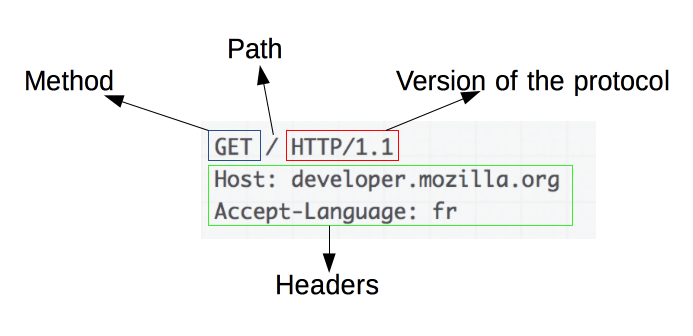
\includegraphics[width=0.7\textwidth]{./images/chapter2/http_request.png}
	\caption[Βασική Δομή ενός αιτήματος http]{Βασική Δομή ενός αιτήματος http}
	\label{fig:http_request}
\end{figure}

\subsection{Μέθοδοι}
\label{subsec:http_methods}

Πιο συγκεκριμένα οι βασικές μέθοδοι που παρέχει το http και οι συνήθεις λειτουργίες τους είναι οι εξής:

\begin{itemize}
	\item \textbf{GET}: παίρνει πληροφορία από τον server
	\item \textbf{POST}: υποβάλλει πληροφορία, προκαλώντας αλλαγές στον τρόπο λειτουργίας του server. Σχετίζεται συχνά με τη δημιουργία πληροφορίας που προηγουμένως δεν υπήρχε 
	\item \textbf{PUT}: όπως και πριν στέλνει πληροφορία στον παραλήπτη υπολογιστή, αλλά αυτή τη φορά επηρεάζει πόρους που ήδη υπήρχαν στο σύστημα. Σχετίζεται συχνά με την τροποποίηση ήδη υπάρχουσας πληροφορίας
	\item \textbf{DELETE}: διαγράφει από το σύστημα του server το συγκεκριμένο πόρο.
\end{itemize}

Αξίζει να σημειωθεί ότι πέρα από τις τέσσερις αυτές βασικές μεθόδους υπάρχουν και άλλες όπως είναι 
η \textbf{PATCH} που αποτελεί ειδική περίπτωση της PUT, η \textbf{HEAD} που αποτελεί ειδική περίπτωση της GET,
καθώς και άλλες που σχετίζονται με τη σύνδεση μεταξύ server και client. Αυτές είναι οι \textbf{CONNECT}, \textbf{OPTIONS} και \textbf{TRACE}.
Καθώς όμως, οι υπόλοιπες αυτές οι μέθοδοι, δεν χρησιμοποιούνται τόσο συχνά στην πράξη, δεν θα αναλυθούν περαιτέρω.

\subsection{Εκδόσεις HTTP}
\label{subsec:http_versions}

Η πρώτη έκδοση του HTTP, παρόλλο που δεν είχε κάποια συγκεκριμένo τίτλο, εκ των υστέρων ονομάστηκε 
HTTP/0.9. Αποτελεί την πιο απλή έκδοση του πρωτοκόλλου. Δεν υποστηρίζονταν headers και κωδικοί κατάστασης (status codes).
Εξυπηρετούσε μόνο GET αιτήματα και η μοναδική απάντηση που μπορούσε να επιστρέψει ήταν hypertext αρχεία. Kάθε φορά που ο server ανταποκρινόταν και έστελνε
απάντηση, η επικοινωνία με τον client έκλεινε κατευθείαν.

Στη συνέχεια και με την ανάπτυξη του διαδικτύου προστέθηκαν και άλλες λειτουργίες. Πέριξ του 1996,
με τη επόμενη έκδοση του πρωτοκόλλου (HTTP/1.0) τα αιτήματα πλέον συνοδεύονταν από headers, μεταπληροφορία σχετικά
με τη κατάσταση του αιτήματος, τον τύπο της πληροφορίας που περιμένουμε να έρθει (stylesheets, media, hypertext) καθώς και 
την έκδοση του HTTP που χρησιμοποιήθηκε στη συγκεκριμένη επικοινωνία. Επιπλέον πέρα από τη GET μέθοδο υπάρχει η
δυνατότητα για POST και PUT, δημιουργία και τροποποίηση πληροφορίας δηλαδή.

Στη συνέχεια το HTTP/1.1 προσπαθεί να βελτιώσει τις ήδη υπαρχουσες δυνατότητες κάνοντας την επικοινωνία
μεταξύ server και client πιο αποδοτική. Αντί να κλείνει η επικοινωνία μετά από κάθε μήνυμα, η σύνδεση παραμένει
ανοιχτή γλιτώνοντας έτσι μία σταθερή καθυστέρηση που υπήρχε σε κάθε αίτημα

Φτάνοντας στο σήμερα, μιλάμε για το HTTP/2.0 \cite{http2}. Αξιοποιώντας το πρωτόκολλο Speedy (SPDY) που αναπτύχθηκε κάποια χρόνια πριν
την κυκλοφορία του, και κτίζοντας πάνω σε αυτό, κατάφερε να μειώσει τους χρόνους επικοινωνίας server-client.
Μερικοί από τους τρόπους που επιτυγχάνεται αυτό είναι η μετατροπή του http από text πρωτόκολλο, σε δυαδικό (binary protocoll), επιτρέποντας έτσι χρήση καλύτερων
και αποδοτικότερων τεχνικών επικοινωνίας. Επιπλέον συμπιέζει τους headers (header compression) καθώς αποτελούν πληροφορία που
επαναλαμβάνεται όταν τα αιτήματα στον server είναι συνεχή. Ο server ακόμα, αποκτά έναν μηχανισμό (server-push) που του
επιτρέπει να προωθεί πληροφορία στον client (στην cache του client συγκεκριμένα), που δεν έχει ζητήσει ακόμα, αλλά βάση αυτού
που αιτήται, μάλλον θα ζητήσει εντός της ιδίας συνεδρίας.

Τέλος, πρέπει να αναφερθούμε στην τελευταία, αν και όχι ακόμα ευρέως διαδεδομένη, έκδοση HTTP/3.0. H βασική διαφορά με τους
πρωκατόχους του είναι ότι αλλάζει το πρωτόκολλο επικοινωνίας που χρησιμοποιεί όλα αυτά τα χρόνια, από TCP (Transfer Communication Protocoll) σε
έναν συνδυασμό UDP (User Datagram Protocoll) και QUIC (Quick UDP Internet Connections), μίας νέας τεχνολογίας που λύνει το πρόβλημα και βελτιστοποιεί τόσο το πρόβλημα 
της ασφάλειας των επικοινωνιών (TLS handshakes), όσο και της απώλειας πληροφορίας που μπορεί να υπήρχε λόγω UDP, πρωτοκόλλου που είναι γνωστό
για την ταχύτερη απόδοσή του σε σχέση με το TCP, αλλά και το γεγονός ότι είναι πιο επιρρεπές σε σφάλματα. Η νέα αυτή έκδοση από τα αποτελέσματα 
του \cite{http3} φαίνεται να έχει ήδη καλύτερους χρόνους σε σχέση με τις παλαιότερες εκδόσεις και ήδη το 28\% του διαδικτύου αξιοποιεί τις δυνατότητές του. 


\subsection{Κωδικοί Κατάστασης}
\label{subsec:http_status_codes}

Οι κωδικοί κατάστασεις (status codes) αποτελούν μέρος της απάντησης του server. Επιτρέπουν στον χρήστη να καταλάβει με μία ματιά αν το αίτημα που έχει κάνει έχει επιστρέψει σωστά, ή έχει γίνει κάποιο λάθος στη μεριά του server.
Υπάρχουν πέντε μεγαλύτερες κατηγορίες που στεγάζουν όλες τις υποπεριπτώσεις αυτών. Πιο συγκεκριμένα:

\begin{itemize}
	\item \textbf{Εύρος 100-199}: Υποδηλώνουν ενημερωτική απάντηση σχετικά με τη λειτουργία του server
	\item \textbf{Εύρος 200-299}: Επιτυχή αιτήματα. 
	\item \textbf{Εύρος 300-399}: Υποδηλώνουν την ανακατεύθυνση του μηνύματος του client. Συνήθως συνοδεύονται από το νέο url στο οποίο πρέπει να αποσταλλεί το αίτημα
	\item \textbf{Εύρος 400-499}: Ανεπιτυχές αίτημα, που οφείλεται στον client. Ένα σύνηθες παράδειγμα είναι η αίτηση πρόσβασης σε προστατευόμενους πόρους χωρίς κάποιου είδους αυθεντικοποίηση, ή χωρίς τα σωστά στοιχεία για αυθεντικοποίηση
	\item \textbf{Εύρος 500-599}: Ανεπιτυχές αίτημα, που οφείλεται στον server. 
\end{itemize}
% \input{./chapters/chapter3_theory/section1_dnn.tex}
% \input{./chapters/chapter3_theory/section2_cnn.tex}
% \input{./chapters/chapter3_theory/section3_sota.tex}
\newevenside
\newevenside

% % chapter 3 = State of the art
% - αναφορά σε commercial και open source projects
% - παράθεση πλεονεκτημάτων της δικής μου υλοποίησης (βασικά εδώ αναφέρουμε τα: 
% (1)infinite scalability και ίσως το γεγονός ότι μπορούμε να (
% (2) κοιτάμε σε μεγάλο βάθος χρόνου για να παρουσιάσουμε "συνολικά στατιστικά", χωρίς αυτό να επιβαρύνει τη βάση μας ή να δυσχαιρένει τη λειτουργία του συστήματος μας). 
% Το γεγονός ότι έχει infinite scalebility μας παρέχει τη δυνατότητα να έχουμε
% (3)όσα 1m intervals θέλουμε και ακόμα τη δυνατότητα να κάνουμε stress test με όσα requests per minute θέλει ο χρήστης.
% Tέλος τα περισσότερα ενώ κάποια από αυτά τασ εργαλεία σου δίνουν τη δυνατότητα να κάνεις customise τα μηνυματα που στέλνεις,
% τα περισσότερα δε σε αφήνουν να τροποποιήσεις τα apis σου.

% commercial products - Better Uptime, Pulsetic, Datadog, Freshping, Hyperping, UptimeRobot
% open souce - Upptime, Uptime Kuma, Cabot, Zabbix, Sensu

% % chapter 4 = Υλοποίηση του συστήματος
% 1η Υλοποίηση - Χρήση απλών schedulers και ενός express server που κρατούσαν όλα τα requests μόνο όσο "ζούσε" ο server.
% 2η Υλοποίηση - Προσθήκη στο προηγούμενο ενός κοινού σημείου (socket.io). Σε αυτή την υλοποίηση θα υπήρχαν 1server με τον οποιό θα "επικοινωνούσε" ο χρήστης και πολλοί server "clients" που θα μιλούσαν με τον αρχικό. Η χρήση websockets/socket.io θα ήταν εξαιρετική, καθώς θα μπορούσε σε κάποιες περιτπώσεις να οφελεί η αμφίφρομη εποικοινωνία server και worker, αλλά το γεγονός ότι οι περισσότερες επικοινωνίες θασ είναι μονόδρομες μάλλον μας ωθεί να χρησιμοποιήσουμε έναν κλασικό http server. Επίσης το scaling ενός websocket server είναι αρκετά πιο περίπλοκο και δύσκολο στη συντήρηση.
% 3η Υλοποίηση - Χρήση ενός ή περισοοτέρων (εφόσον χρειαστεί) server και ένας ή περισσότερη workers (scalable). Η κεντρικός server εξυπειρετεί μόνο την επικοινωνία μεταξύ worker και χρήστη και είναι υπεύθυνος για τη δημιουργία, καταστροφή, τροποποίηση ήδη υπάρχοντων jobs. Κάθε worker έχει το δικό του scheduler και εκτελεί τα δικά του jobs/apis καθώς και ένα cleanup jobs μία φορά τη βδομάδα που κάνει Upload τα raw responses, κάποια χρήσιμα στοιχεία σε ξεχωριστά αρχεία καθώς και υπολογίζει/επαναυπολογίζει χρήσιμες στατιστικές τιμές για κάθε μέρα (εδώ αναφορά στο πως περίπου λειτουργεί ο scheduler και εξήγηση της λειτουργίας του άμα "πέσει")

% % chapter 5 = Επίδειξη Συστήματος
% - Παρουσίαση εικόνων από website
% - Εξήγεισαι τι δείχνουν και λειτουργικότητα

\newevenside
%\newevenside

\renewcommand{\bibname}{Βιβλιογραφία}
\bibliography{./bibliography/chapter1.bib, ./bibliography/chapter2.bib}

\end{document}

